With the increasing number of cores per processor, having an SMP architecture becomes tough.
To accommodate more cores per processors Non Uniform Memory Architecture (NUMA) came into existence.
NUMA acrhitecture has proved to be scalable with increasing number of cores.
But the physical arrangement of the processors on the chip, so that they are equidistant from each other is a tough problem.
Due to which there are varied distances between different pairs of processors.
This gives rise to various combinations of memory and thread placement, resulting into varied data access costs.
Having said that, the next problem is the optimistic scheduling of threads and data.

A typical NUMA machine has Nodes connected to each other via bus called as interconnect.
Each node hosts few number of cores, each having their own L1 and L2 caches, and a L3 cache shared by all the cores.
Along with a full hierarchy of caches, each node is allocated a seperate memory.

Work described in \cite{Majo:2011:MMN:1993478.1993481} has shown the penalties of data access across inteerconnect and proposed a NUMA aware scheduler.
Figure \ref{fig:numaMatrix} shows a penalty matrix in terms of data fetch overhead for the AMD Opteron machine we have used for our experiments.
We placed the data on one node and let threads placed on all four nodes to modify that data.
For example, in the first row, Node N0 holds the data and all four nodes, N0, N1, N2, N3 have threads modifying the data.
The values show the slowdown experienced by different threads due to interconnect.
Node N0 takes unit time as it is local to data, Node N1 and N2 experience 33\% slowdown as they are accessible via single hop, and node N3 shows 66\% overhead as it is accessible via 2 hops.
We have repeated the experiment by placing data on each of the other three nodes, to get a full matrix indicating distance between any two processors.

\begin{figure}
    \centering
    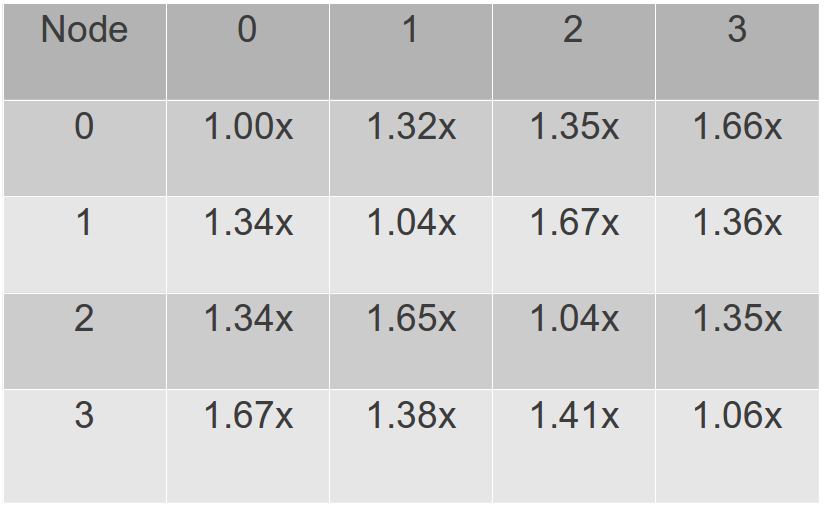
\includegraphics[scale=0.35]{numaMatrix.png}
    \caption{This shows the slowdown between each node. }
    \label{fig:numaMatrix}
\end{figure}

